\section{Early detection of potential dropout students}

\label{sec:strategy}

This way, the problem we address in this paper consists of a strategy to \textit{early} identify potential failing students. Notice that identifying early is very important in the sense that professors still have enough time to act and avoid students to fail the course. This way, we focus exclusively on early identifying these students. Providing or reporting a technique useful to reduce the failure rate is outside the scope of this paper. Nevertheless, notice that when identifying them we may study the data and afterwards provide a technique to do so. Actually, based on the results of this paper, we intend to propose a technique to reduce the failure rate as future work.

Next, we detail our strategy to identify these students.

\subsection{Online judge system}
% This section should answer: Why is this kind of system important to identify potential falling students?
% Answer: We need metrics. In order to discover how students are performing, it is necessary a close monitoring of students behaviour
% Talk about Huxley, only enough to explain the metrics: submissions and submission_status (Correct ...)
In order to discover how students are performing, it is important to define a strategy to close monitoring students’ behavior. This strategy should include a way to extract metrics from students. Online learning tools may be a source for these metrics. In the context of programming, a very popular category of systems is the online judges. These systems present students to a set or programming problems. The students solve the problem using a programming language and then submits their solutions. The online judge runs the student’s solution against a set of test cases and in the case the solution passes over all the tests it will be evaluated as correct, otherwise, it will be evaluated according to the type of error, such as wrong answer, compilation error, runtime error, etc.

% Why the Huxley and not others?
% answer: Metrics and performance improvement (not in scope)
In our strategy, we choose to use an online judge named \emph{The Huxley} \cite{paes2013ferramenta} to collect metrics from our students. In this system, the judge provides one of the following outputs for a submission: correct, wrong answer, time limit exceeded, compilation error, runtime error, presentation error and empty answer. We will use these outputs as the main source of metrics. This particular online judge system was chosen because it has some features that we believe will be useful to improve the overall performance of students as a future direction of this research. More specifically, the tool will support us to deal with the following problems:
\begin{itemize}
  \item Students only learn how to program by programming~\cite{jenkins-ltsn02}. The Huxley provides a database composed of more than 300 problems. It allows students to submit their solutions to any of these problems and they are encouraged to try once mistakes are not penalized.
  \item Sometimes a student who misses a basic concept and then cannot follow the next lecture. She believes that there is no going back; the course is behaving is a speed that she thinks she will be not able to follow. Such a student will quickly come to the view that ``they just cannot do programming'', and will attribute this to the perceived difficulty of the subject. In other words, students learn at different speeds. As the tools is available online on the Internet, each student can find its own rhythm on an extra class schedule.
  \item Students need rapid feedback. Many professors are overwhelmed with their daily activities. Then they have no time to give feedback on every student code. On the other side, students need this feedback to continue their learning process in the right path. The Huxley provides a feedback right after the student submits her code. The feedback indicates whether user produces the right answer and gives tips in the case user otherwise.
  \item There always be great students and bad students. The great ones should be presented to challenges that make them even greater and the bad ones should be presented to a different set of problems that allow them to become better. Each programming problem of the Huxley is classified according to this level of difficulty and the programming topics it covers. This allows each student to choose the next problem in accordance with this level of expertise.
\end{itemize}

\subsection{Metrics}

\label{sec:metrics}

We use two metrics in our strategy. We explain them in what follows:

\begin{itemize}

	\item \textbf{Number of submissions:} this metric represents the number of submissions a student do during the course. As explained, Huxley provides more than 300 programming exercises. To solve a particular problem, a student needs to submit at least one solution.

	\item \textbf{Number of correct submissions:} if a student solves one problem, we increase this metric by one.

\end{itemize}

Depending on the level of difficulty of a problem, students may submit several times to solve it. However, notice that this is not necessarily a bad thing regarding the learning process. For example, submitting many times means that students are somehow practicing and studying continuously. Thus, although she is not hitting a right solution, she is trying hard and will eventually hit one. Nevertheless, we need to carefully analyze \todots

\todo{Por que essas metricas sao boas? Por que escolhemos elas? O texto acima ajuda a explicar isso? Essas metricas nao sao obvias?}

\subsection{Clustering algorithm}

To identify potential failing students, we use the well-known clustering algorithm k-means~\cite{}. As input, we set the algorithm to compute three groups. To compute the groups, the algorithm takes into account the metrics we present in Section~\ref{sec:metrics}.

We choose three groups because ???

\todo{Por que escolhemos clustering? Por que o k-means?}

\todo{Por que 3 grupos? O do meio seria impossível prever algo. Mas isso nao e obvio?}

\subsection{Summary}

Figure~\ref{fig:strategy} combines all steps of our strategy. As the classes are happening, students are encouraged to solve exercises using the problems of The Huxley. Although solving exercises is not mandatory, there are some particular activities where the professor forced students to use The Huxley. Next, we collect the metrics we detailed in Section~\ref{sec:metrics}. Then, we execute a R script we implemented to execute the clustering algorithm. As can be seen, there are three groups, represented by circles, squares, and stars. \todo{falar dos 30 dias}

\begin{figure}[htb]
\centering
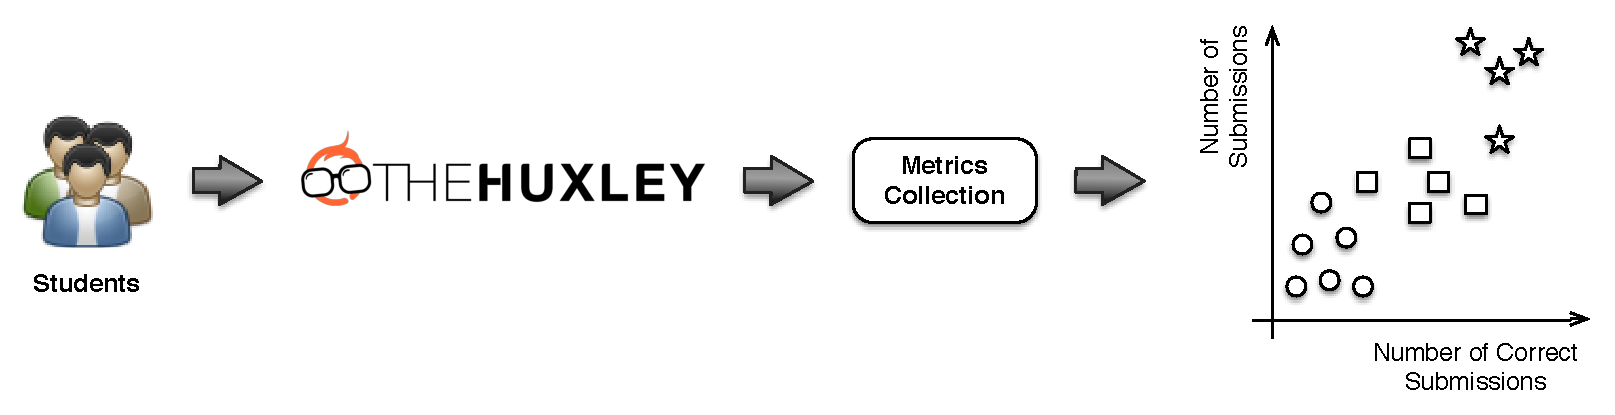
\includegraphics[width=1.0\textwidth,natwidth=610,natheight=642]{images/Strategy.pdf}
\caption{Summary of our strategy to identify potential failing students.}
\label{fig:strategy}
\end{figure}

Now, according to the groups, we have the potential failing students, the ones that have a small number of submissions and correct submissions (represented by circles). Notice we also have students that are potential candidates to successfully pass (represented by stars): after 30 days, they seem to be studying hard, due to the high number of submissions.

After applying the clustering algorithm, we need to check if the algorithm correctly predicted the failing students. To do so, we use the academic system of the Federal University of Alagoas to look for grades and check whether the students passed or not. For example, for the detached star, the algorithm pointed it right: after 30 days, it identified the student would pass and she did. The same happened for the detached circles: after 30 days, the algorithm pointed that both students would not pass and they did not. Nevertheless, notice that our strategy is susceptible to false positives (the algorithm pointed the student would pass, but she did not) and false negatives (the algorithm pointed the student would not pass, but she did). We shall consider and discuss these cases in Section~\ref{}.

After confronting the algorithm results with the academic system, we perform some statistics.

\todo{essa parte da estatistica nao eh a estrategia. Tem que separar as coisas! Sera que essa figura esta com cara de explicar a avaliacao?} 